%%%%%%%%%%%% Attribution %%%%%%%%%%%%
% This template was created by 
% Chuck F. Rocca at WCSU and may be
% copied and used freely for 
% non-commercial purposes.
% 10-17-2021
%%%%%%%%%%%%%%%%%%%%%%%%%%%%%%%%%%%%%

%%%%%%% Start Document Header %%%%%%%
% In creating a new document
% copy and paste the header 
% as is.
%%%%%%%%%%%%%%%%%%%%%%%%%%%%%%%%%%%%%

\documentclass[12pt]{article}

%%%% Header Information %%%%
    %%% Document Settings %%%%
    \usepackage[utf8]{inputenc}
    \usepackage[
        twoside,
        top=1in,
        bottom=0.75in,
        inner=0.5in,
        outer=0.5in
    ]{geometry}
    \pagestyle{myheadings}

%%%% Additional Commands to Load %%%%
    \usepackage{tcolorbox}
    \tcbuselibrary{skins}
    \usepackage{minted}
    \usepackage{color}
    \usepackage{tikz}
    \usetikzlibrary{calc}
    \usepackage{tabularx,colortbl}
    \usepackage{amsfonts,amsmath,amssymb}
    \usepackage{titling}
    \usepackage{mathrsfs}
    \usepackage{calc}
    \usepackage{xepersian}

%%%% Commands to Define Homework Boxes %%%%
%%%% Box Definition %%%%
    \newtcolorbox{prob}[1]{
    % Set box style
        sidebyside,
        sidebyside align=bottom,
    % Dimensions and layout
        width=\textwidth,
        toptitle=2.5pt,
        bottomtitle=2.5pt,
        righthand width=0\textwidth,
    % Coloring
        colbacktitle=gray!30,
        coltitle=black,
        colback=white,
        colframe=white,
    % Title formatting
        title={
            #1 \hfill نمره:\phantom{WWWW}
        },
        fonttitle=\large\bfseries
    }

%%%% Environment Definition %%%%
    \newenvironment{problem}[1]{
        \begin{prob}{#1}
    }
    {
        \tcblower
        \centering
        \vspace{\baselineskip}
        \end{prob}
    }



%%%% Document Information %%%%
    \title{\lr{HW3 Solutions}}
    \date{}
    \author{\lr{Written by Reza Shahriari}}
    \usepackage{amsmath}

%%%%%%% End Document Header %%%%%%%


%%%% Begin Document %%%%
% note that the document starts with
% \begin{document} and ends with
% \end{document}
%%%%%%%%%%%%%%%%%%%%%%%%
\settextfont{BNAZANIN.TTF}

\begin{document}

%%%% Format Running Header %%%%%
\markboth{\theauthor}{\thetitle}

%%%% Insert the Title Information %%%
\maketitle


%%%% General Description of the Document %%%%



%%%% Introduction to the General Template %%%%
\section{بخش اجباری}
\centering
\lr{Disclaimer:} 

\lr{This is the solution manual to the homework assigned to students of Digital Control - Dr.Talebi.}

\lr{We do not guarantee that this solution is precise and thorough so please contact your TA to propose your innovative solutions and/or any probable mistakes.}

    \begin{problem}{سوال اول}
    	\raggedleft
    	\lr{First draw the original SFG :}
    	
    	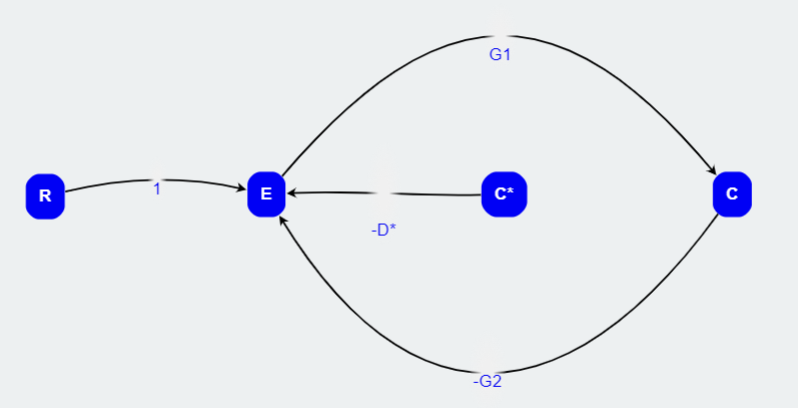
\includegraphics[width=\linewidth]{Resources/5.png}
    	
    	$C = G_1E$
    	
    	$E = R - G_2C - D^*C^*$
    	
    	$C = \frac{G_1R}{G_1G_2+1} - \frac{D^*C^*}{1+G_1G_2} $
    	
    	\lr{Derive $C^*$ as follows:}
    	
    	$C^* = (\frac{G_1R}{1+G_1G_2})^* - (\frac{1}{1+G_1G_2})^*D^*C^*$
    	
    	$C^* = \frac{(\frac{G_1R}{1+G_1G_2})^*}{(1+ (\frac{1}{G_1G_2})^*D^*)}$
    	
    	$C = \frac{G_1R}{G_1G_2+1} - \frac{D^*(\frac{(\frac{G_1R}{1+G_1G_2})^*}{(1+ (\frac{1}{G_1G_2})^*D^*)})}{1+G_1G_2} $
    

    \end{problem}
    
    \begin{figure}
    	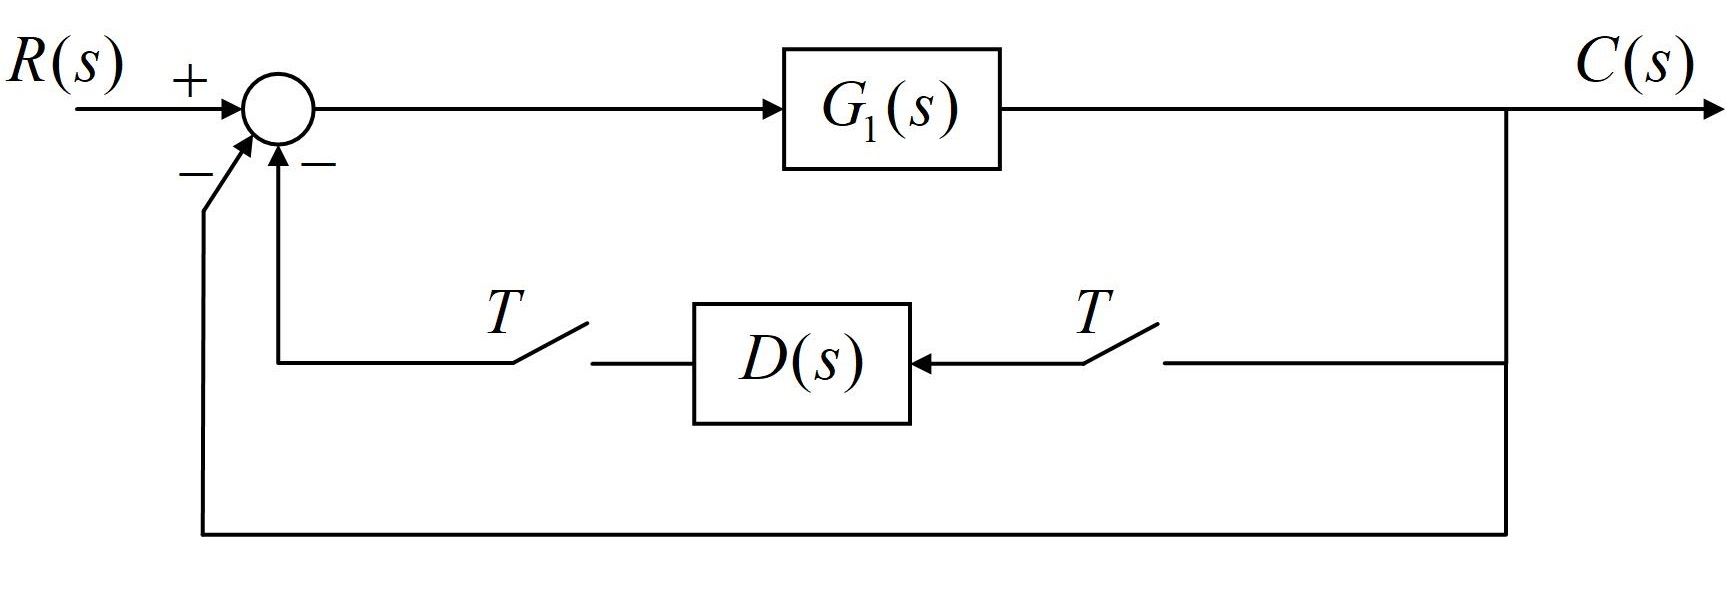
\includegraphics[width=\linewidth]{Resources/3.png}
    	\caption{شکل سوال اول}
    \end{figure}
    
    \begin{problem}{سوال دوم}
    		\raggedleft
    	\lr{Recall the equivalent for forward discretization :}
    	
    	$s\to \frac{z-1}{T}$
    	
    	\lr{we must substitute it in the transfer function to get the following discrete transfer function:}
    	
    	$H{{(z)}_{forward}}=10\frac{z-0.75}{z+1.5}$
    	
    	\lr{from the original transfer function we have:}
    	
    	$
    	\frac{s+1}{0.1s+1}\xrightarrow{s\to j\omega }\frac{j\omega +1}{0.1j\omega +1}  
    	\frac{j\omega +1}{0.1j\omega +1}=\frac{\sqrt{{{\omega }^{2}}+1}}{\sqrt{{{(0.1\omega )}^{2}}+1}}\angle {{\tan }^{-1}}\omega -{{\tan }^{-1}}0.1\omega
    	$
    	
    	$
    	\omega =3\to \varphi ={{\tan }^{-1}}3-{{\tan }^{-1}}0.3\simeq {{55}^{\circ }}
    	$
    	
    	$
    	H{{(z)}_{forward}}=10\frac{z-0.75}{z+1.5}\xrightarrow{z={{e}^{j\omega T}}}10\frac{{{e}^{j\omega T}}-0.75}{{{e}^{j\omega T}}+1.5} 	 
    	$
    	
    	$
    	10\frac{\cos \omega T-0.75+j\sin \omega T}{\cos \omega T+1.5+j\sin \omega T}
    	$
    	
    	$  
    	\varphi ={{\tan }^{-1}}\frac{\sin \omega T}{\cos \omega T-0.75}-{{\tan }^{-1}}\frac{\sin \omega T}{\cos \omega T+1.5}
    	$
    	
    	$  
    	\varphi ={{\tan }^{-1}}\frac{\sin 0.75}{\cos 0.75-0.75}-{{\tan }^{-1}}\frac{\sin 0.75}{\cos 0.75+1.5}	 
    	$
    	
    	$
    	\varphi ={{\tan }^{-1}}\frac{.68}{.0183}-{{\tan }^{-1}}\frac{0.68}{0.23168}=88.46 - 16.94 = 71.52
    	$
    	
    	\lr{Discretize using the Backward rule to get :}
    	
    	$s\to \frac{z-1}{Tz}$
    	
    	$H{{(z)}_{Backward}}=3.57\frac{z-0.8}{z-0.286}$
    	
    	$
    		 H(z)=3.57\frac{z-0.8}{z-0.286}\xrightarrow{z\to {{e}^{j\omega T}}}3.57\frac{{{e}^{j\omega T}}-0.8}{{{e}^{j\omega T}}-0.286}
    	$	 
    	
    	$	  
    		3.57\frac{\cos \omega T-0.8+j\sin \omega T}{\cos \omega T-0.286+j\sin \omega T}
    	$
    	
    	 
    	$	 \varphi ={{\tan }^{-1}}\frac{\sin \omega T}{\cos \omega T-0.8}-{{\tan }^{-1}}\frac{\sin \omega T}{\cos \omega T-0.286} 
    	$
    	
    	$
    		 \varphi ={{\tan }^{-1}}\frac{\sin 0.75}{\cos 0.75-0.8}-{{\tan }^{-1}}\frac{\sin 0.75}{\cos 0.75-0.286}	 
    	$
    	
    	$ 
    		 \varphi ={{\tan }^{-1}}\frac{0.68}{0.0683}-{{\tan }^{-1}}\frac{0.68}{0.4457} 
    	$
    	
    	$ 
    		 \varphi \simeq 40
    	$

    \end{problem}
    
    \begin{problem}{سوال سوم}
    	\raggedleft
    	\lr{Recall the formula for tustin with prewarping:}
    	
    	$s\to \frac{1}{\tan (\frac{{{\omega }_{1}}T}{2})}\frac{z-1}{z+1}$
    	
    	\lr{we must substitute it in the transfer function to get the following discrete transfer function:}
    	
    	$H(z)=4.89\frac{z-0.768}{z-0.161}$
    	
    	$
    		H(z)=4.89\frac{z-0.768}{z+0.161}\xrightarrow{z\to {{e}^{j\omega T}}}4.89\frac{{{e}^{j\omega T}}-0.768}{{{e}^{j\omega T}}+0.161} 
    	$
    	
    	$ 
    		4.89\frac{\cos \omega T-0.768+j\sin \omega T}{\cos \omega T+0.161+j\sin \omega T}
    	$
    	
    	$ 
    		\varphi ={{\tan }^{-1}}\frac{\sin \omega T}{\cos \omega T-0.768}-{{\tan }^{-1}}\frac{\sin \omega T}{\cos \omega T+0.161}
    	$
    	
    	$ 
    		\varphi ={{\tan }^{-1}}\frac{0.68}{.0363}-{{\tan }^{-1}}\frac{0.68}{0.8926}
    	$
    	
    	$ 
    		\varphi =-86.944-37.3
    	$
    	
    	$ 
    		\varphi =55.756 
    	$
    	
    \end{problem}
    
    
    \begin{problem}{سوال چهارم}
    	\raggedleft
    	\lr{Recall the equivalent formula for zero pole matching. Substitute it to get the discrete transfer function as bellow:}
    	
    	${{H}_{PZ}}=4.150\frac{z-0.779}{z-0.082}$
    	
    	$
    		{{H}_{PZ}}=4.150\frac{z-0.779}{z-0.082}\xrightarrow{z\to {{e}^{j\omega T}}}4.150\frac{{{e}^{j\omega T}}-0.779}{{{e}^{j\omega T}}-0.082}
    	$
    	
    	$
    		4.150\frac{\cos \omega T-0.779+j\sin \omega T}{\cos \omega T-0.082+j\sin \omega T}
    	$
    	
    	$
    		\varphi ={{\tan }^{-1}}\frac{\sin \omega T}{\cos \omega T-0.779}+{{\tan }^{-1}}\frac{\sin \omega T}{\cos \omega T-0.082} 
    	$
    	
    	$
    		\varphi ={{\tan }^{-1}}\frac{0.68}{-0.047}-{{\tan }^{-1}}\frac{0.68}{0.6496}
    	$
    	
    	$
    		\varphi =-86.046-46.3097
    	$
    	
    	$
    		\varphi =47.64
    	$
    \end{problem}
    
    \begin{problem}{سوال پنجم}
    	\raggedleft
    	\lr{Looking back at the calculations of section 4.3.3 of Digital Control of Dynamic Systems by G.Franklin:}
    	
    	\lr{Let's choose T=1}
    	
    	\begin{align}
    		& x(k+1)=\Phi x(k)+\Gamma u(k) \nonumber \\ 
    		& y(k)=Hx(k)
    	\end{align}
    	
    	\begin{align}
    		& \Phi ={{e}^{AT}} \nonumber \\ 
    		& \Gamma =\int\limits_{0}^{T}{{{e}^{A\eta }}d\eta }B \nonumber \\ 
    		& \Phi ={{L}^{-1}}\left\{ {{\left( sI-AT \right)}^{-1}} \right\} \nonumber \\ 
    		& AT=\left( \begin{matrix}
    			0 & 1  \nonumber\\
    			-1 & -1 \nonumber \\
    		\end{matrix} \right) \nonumber\\ 
    		& \Phi ={{L}^{-1}}\left\{ \left( \begin{matrix}
    			\frac{s+1}{{{s}^{2}}+s+1} & \frac{-1}{{{s}^{2}}+s+1}  \nonumber\\
    			\frac{1}{{{s}^{2}}+s+1} & \frac{s+1.57\times {{10}^{-16}}}{{{s}^{2}}+s+1}  \nonumber\\
    		\end{matrix} \right) \right\} \nonumber
    	\end{align}
    	
    	\lr{The rest is routine and left as an exercise to students.}
    	
    		 
    
    	

    \end{problem}
    
    \begin{problem}{سوال ششم}
    \raggedleft
    \lr{Follow section 6.1 , equations 6.27 through 6.31 of Digital Control of dynamic systems by G.Franklin for the solution.}
	
	\end{problem}    
    
\raggedleft
\section{بخش امیتازی}
    \begin{problem}{سوال هفتم}
    	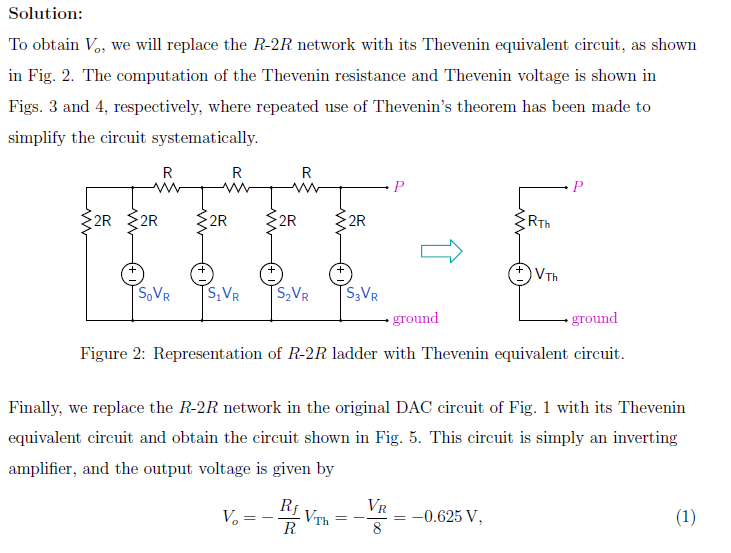
\includegraphics[width=\linewidth]{Resources/4.png}
	
	
	\end{problem}   
	\begin{figure}
		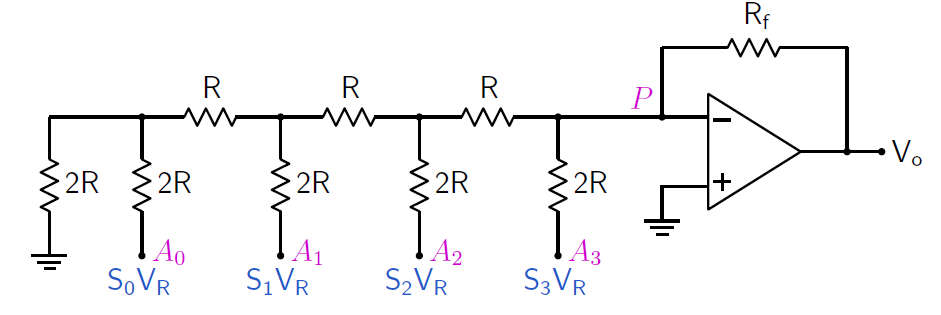
\includegraphics[width=\linewidth]{Resources/1.png}
		\caption{شکل سوال هفتم}
	\end{figure}
    \begin{problem}{سوال هشتم}
    	\raggedleft
    	\lr{This task must be done in multiple steps:}
    	
    	\lr{Firstly, compare 10 which is half of 20 with the input voltage:}
    	
    	$10 < 13.478$ 
    	
    	\lr{MSB Gets Set we have : 10000000}
    	
    	$10 + 5 > 13.478$ 
    	
    	\lr{the next bit remains 0 : 10000000}
    	
    	$10+2.5 < 13.478$ 
    	
    	\lr{the next bit gets set : 1010000}
    	
    	$10+2.5+1.25 > 13.478$ 
    	
    	\lr{the next bit remains 0 : 10100000}
    	
    	$10 + 2.5 + 0.625 < 13.478$ 
    	
    	\lr{the next bit gets set : 10101000}
    	
    	$10 + 2.5 + 0.625 + 0.3125 < 13.478$ 
    	
    	\lr{the next bit gets set : 10101100}
    	
    	$10 + 2.5 + 0.625 + 0.3125 + 0.15625$ 
    	
    	\lr{the next bit remains 0 : 10101100}

	
	
	
	\end{problem}
	\begin{figure}
		\centering
		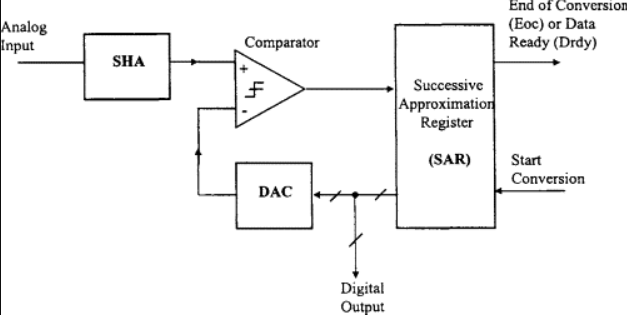
\includegraphics[scale=0.7]{Resources/2.png}
		\caption{شکل سوال هشتم}
	\end{figure}

\end{document}
